\documentclass[10pt,twocolumn]{article}

% use the oxycomps style file
\usepackage{oxycomps}
\usepackage{graphicx}

% usage: \fixme[comments describing issue]{text to be fixed}
% define \fixme as not doing anything special
\newcommand{\fixme}[2][]{#2}
% overwrite it so it shows up as red
\renewcommand{\fixme}[2][]{\textcolor{red}{#2}}
% overwrite it again so related text shows as footnotes
%\renewcommand{\fixme}[2][]{\textcolor{red}{#2\footnote{#1}}}

% read references.bib for the bibtex data
\bibliography{references}

% include metadata in the generated pdf file
\pdfinfo{
    /Title (Reinforcement Learning Tutorial)
    /Author (James Derrod)
}

% set the title and author information
\title{Reinforcement Learning Tutorial}
\author{James Derrod}
\affiliation{Occidental College}
\email{jderrod@oxy.edu}

\begin{document}

\maketitle

\section{Introduction}
    I am very interested in artificial intelligence and plan to do my comps project on training an artificial intelligence to accomplish a designated task. The tutorial that I did to learn about this used OpenAI's open source tool for training artificial intelligence, Gym, which is now being maintained by The Farma Foundation and has been renamed to Gymnasium.\cite{FrozenLake}\cite{FrozenLakeTutorial} \cite{InstallTutorial}

    The goal of this tutorial is to train a neural network to successfully accomplish its assigned task, in this case, avoid all obstacles while finding and reaching the goal efficiently, without prior knowledge of the environment.

\section{Methods}

    
    To begin setting up the environment our agent will interact with, first instantiate the FrozenLake-v1 environment. This simulated environment consisted of a grid with 64 potential states, laid out in an 8x8 matrix, where each state represented a unique location on the grid. The agent's movements were constrained to four cardinal actions: moving left, moving downwards, right, or upwards, with each action transitioning the agent to a different state on the grid.

    \begin{figure}[ht]
    \centering
    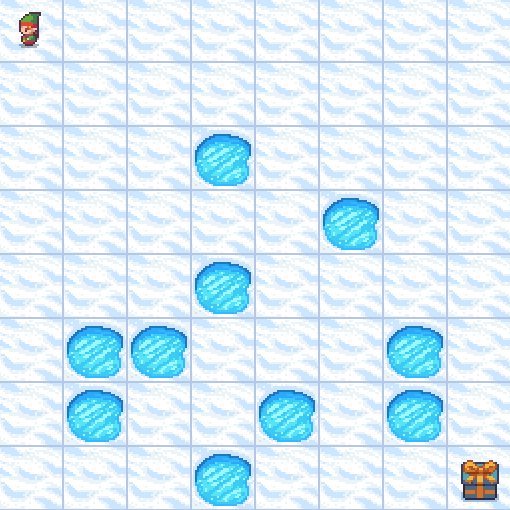
\includegraphics[width=0.70\linewidth]{FrozenLake8x8.PNG}
    \caption{Render of FrozenLake environment.}
    \label{fig:frozenlakeenv}
    \end{figure}
    
    
    Adding to the complexity, the feature termed 'slippery condition' has been enabled, a critical component of our environment setup. This feature introduced an element similar to walking on actual ice, where the likelihood of the agent slipping into a non-intended direction was a built-in uncertainty. This particular aspect was designed to make the environment more challenging and realistic.

    In terms of the reward system, the structure was designed to be binary for simplicity. The agent would receive a reward of one upon successfully navigating to the goal, simulating the completion of the task. There were no intermediate rewards throughout the journey on the grid, allowing the agent's motivation to be singularly focused on reaching the target location. The lack of intermediate rewards meant that the only metric for success was whether the goal had been reached, setting a clear and definitive outcome for the agent's learning process.
    
    
    Q-learning is a model-free reinforcement learning algorithm that enables an agent to learn the value of an action in a particular state. It works by estimating the rewards an agent can expect for each action at each state, helping the agent to make decisions that maximize these rewards over time. The algorithm updates its estimates using the formula that incorporates the learning rate, discount factor, and the maximum future rewards. This process continues until the agent's policy converges to the optimal policy that dictates the best action at each state.

    
    In the FrozenLake environment, Q-learning is employed to train our agent to navigate the grid by learning to avoid holes and reach a goal. The algorithm updates a Q-table, which represents the expected rewards for actions taken in each state, using experiences gained through interaction with the environment. For this environment, the Q-table would consist of 64 rows, and 4 columns, 1 row for every state and one column for each possible action at each state. This learning process is guided by the balance between exploring new actions and exploiting known ones to maximize rewards, ultimately aiming to find the optimal path across the lake with the complexities introduced by the 'slippery' condition of the ice.

    Carefully selected key parameters optimize the Q-learning algorithm's effectiveness. The learning rate (alpha) was set to 0.9, influencing the speed at which the agent incorporates new information. The discount factor (gamma), also set at 0.9, determines the importance of future rewards, balancing the agent's short-term and long-term benefits. The epsilon-greedy policy was employed to balance exploration and exploitation, starting with a 100\% exploration rate (epsilon = 1) and gradually decreasing to encourage exploitation of learned behaviors.

    
    In the training loop, the agent repeatedly interacts with the FrozenLake environment to learn the optimal actions. At each iteration, it either explores by choosing an action randomly, based on the epsilon value, or exploits known information by selecting the action with the highest Q-value for its current state. After executing an action, the agent observes the reward and new state, which it uses to update the Q-table. This loop continues across episodes, gradually reducing epsilon to shift from exploration to exploitation, refining the agent's strategy over time.
    
    As training episodes unfolded, Q-values, representing the expected utility of actions in each state, gradually refined to reflect more optimal decision-making paths. The agent's policy improvement was evident through its increasingly successful navigation towards the goal, minimizing falls into holes. This progress was further quantified by tracking the frequency of reaching the goal, with improvements in Q-values correlating with higher success rates.

    While Q-learning proved to be a suitable approach for our FrozenLake project, there are other reinforcement learning methods that could have been considered. These include Deep Q-Networks (DQN), which combine Q-learning with deep neural networks, Policy Gradient methods, and Actor-Critic methods that utilize both value and policy-based techniques.

    Deep Q-Networks, for instance, could handle more complex state spaces due to their deep learning capabilities but may be an over extension for the relatively simple environment of FrozenLake. Policy Gradient methods, on the other hand, could provide more nuanced policies but at the cost of increased computational complexity and potentially more instability in training. Lastly, Actor-Critic methods, while powerful, require fine-tuning and balancing two different architectures, which can be challenging and time-consuming.

    I've opted for vanilla Q-learning due to its simplicity, transparency, and ease of implementation, which aligns well with the discrete state and action spaces of the FrozenLake environment. The effectiveness of this method is validated by the clear learning progression and success rate demonstrated by the agent, as reflected in the results section.

\section{Metrics \& Results}

    To determine if we've successfully trained the neural network as intended, we gauge its proficiency in avoiding obstacles and reaching the goal efficiently. This efficiency is quantified by observing the network's success rate across numerous runs. A rising trend in this rate would indicate an increasingly adept neural network, learning to navigate the challenges of the FrozenLake environment. The measure of success lies in the consistency and reliability of the agent's performance. The upward trend not only confirms the agent's improving capability but also validates the effectiveness of the Q-learning algorithm in teaching the neural network to understand and react to the environment without prior knowledge.

    \begin{figure}[ht]
    \centering
    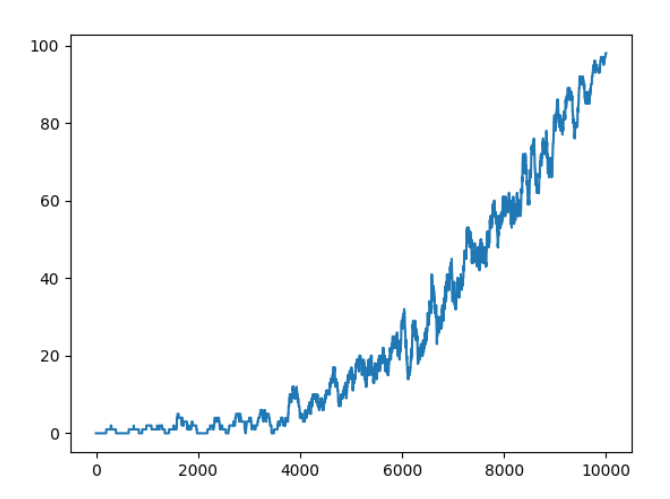
\includegraphics[width=0.75\linewidth]{rl_success.PNG}
    \caption{Success rate of the AI agent across runs, indicating the likelihood of reaching the goal in each trial.}
    \label{fig:successrate}
    \end{figure}

    
    The trend observed in the graph following the success rate of our AI agent indicates an exponential learning curve. Initially, the agent's performance shows gradual improvement, which accelerates as it gains experience. Early on, the increments are quite small, indicating the agent is initially learning slowly. As learning progresses, the improvements in performance become more pronounced, showing the agent is learning more quickly from its accumulated experience. This is typical of many reinforcement learning scenarios where early exploration leads to a rapid accumulation of valuable knowledge once initial patterns are identified. The steepening curve is reflective of the compounding knowledge the agent acquires, showcasing a rapid increase in its problem-solving abilities as it approaches mastery of the task. This exponential trend is a hallmark of effective learning, tracking the agent's growing proficiency in leveraging past insights to navigate new challenges efficiently.

    Aside from the success rate over runs, other metrics could have included:
    \begin{itemize}
        \item Average Reward per Episode: This metric would average the rewards the agent collects in each episode, giving insight into its consistency. It wasn't chosen because our environment only provides a reward upon successfully reaching the goal, making the average reward and success rate closely related.
        \item Convergence Time: The number of episodes required for the Q-values to stabilize, indicating the agent has learned an optimal policy. We focused on the success rate trend over explicit convergence measurement since it more directly reflects performance improvements.
        \item Steps per Episode: The count of steps the agent takes to reach the goal in each episode could provide insights into the efficiency of the learned policy. It was not used as the primary metric as it can be inversely related to exploration, which is an essential part of early learning.
    \end{itemize}

    Each of these metrics offers valuable information but might require additional context to interpret correctly. The success rate alone was a straightforward and intuitive reflection of the agent's learning progression and ultimate performance in achieving the set goal.


\section{Reflection}
    I feel after completing this tutorial that I have learned the foundation of reinforcement learning and am very excited and interested to implement this in other environments. I am still very interested in continuing this topic for my comps project. 
    
    I am concerned about the level of difficulty of building a custom environment, and also that my chosen environment may either be too complex or too simple.
\printbibliography

\end{document}
